El administrador del Departamento de Apoyo Técnico modifica la información de un usuario previamente buscado en la plataforma.

\subsection{Subpaso 2-A: Modificar usuario}
\begin{enumerate}
	\item Ingrese los nuevos datos en la interfaz
    \textbf{IUGS-20 Modificar usuario}, es decir: nombre, primer apellido, tipo de usuario, nivel de usuario, institución, rol, identificador, teléfono, correo electrónico, estado.

    \begin{figure}[hbtp]
	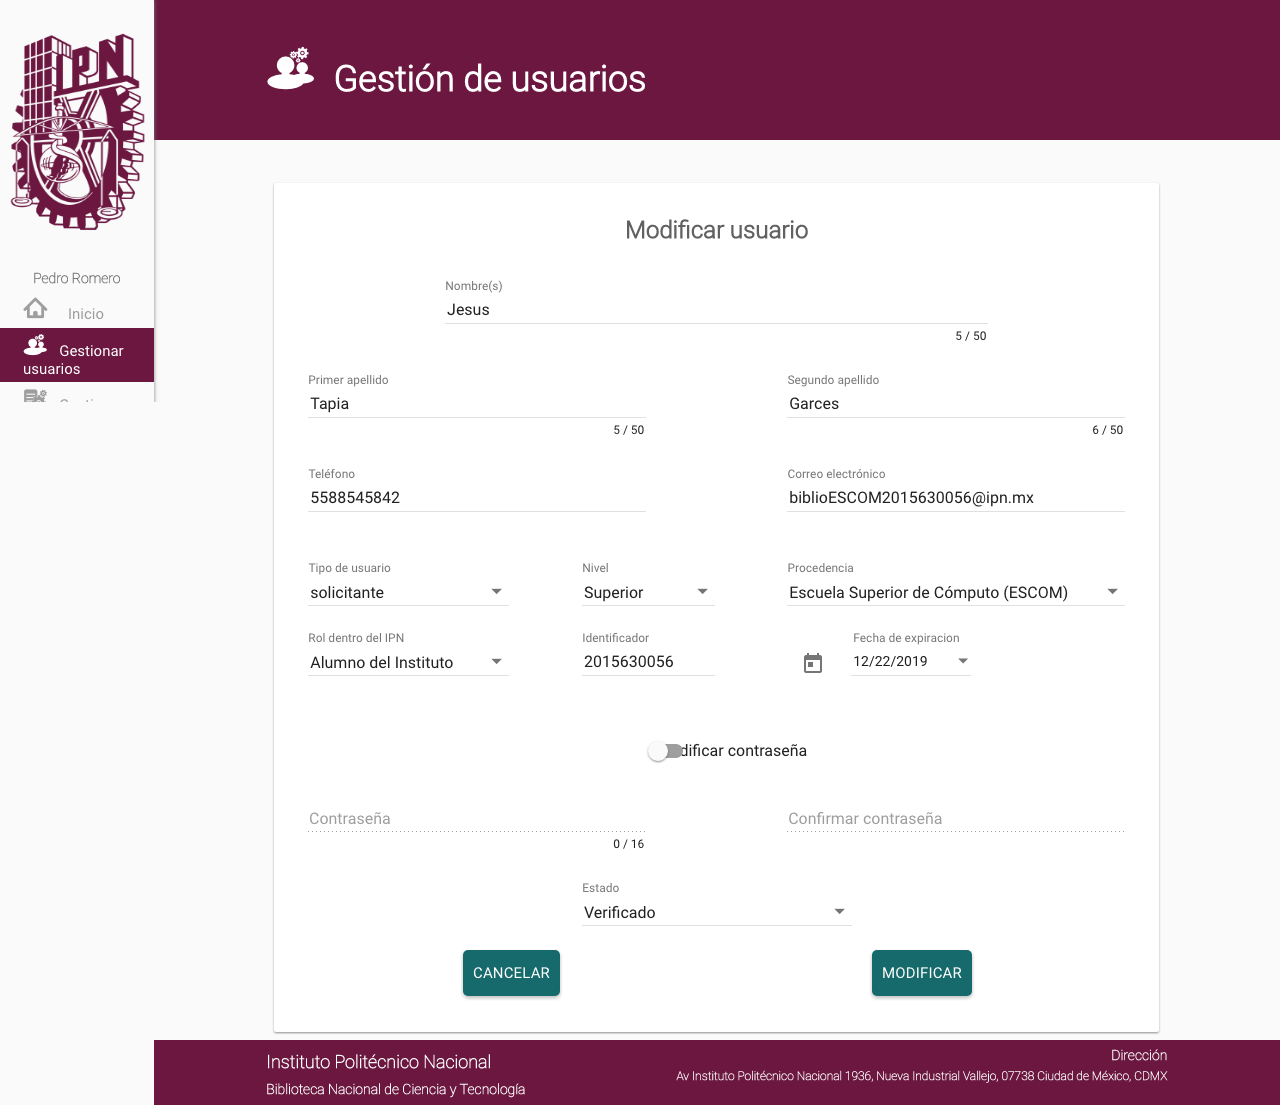
\includegraphics[scale=0.3]{images/Interfaz/IUGS-20 Modificar usuario.png}
	\caption{Modificar usuario}
	\end{figure}

\item Presione el botón \textbf{Guardar cambios}.
\item Presione el botón \textbf{Aceptar} en el mensaje emergente
\textbf{MAT-09 Datos actualizados}.

\begin{figure}[hbtp]
	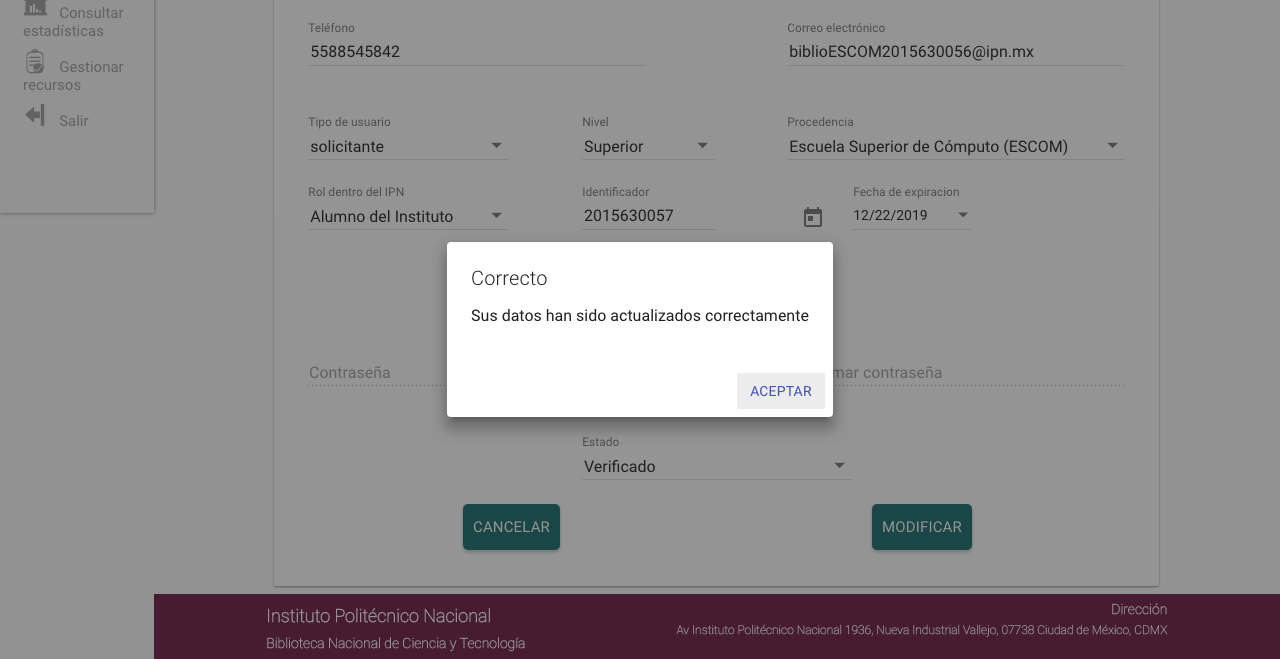
\includegraphics[scale=0.3]{images/Interfaz/MAT-09 Datos actualizados.png}
	\caption{Datos actualizados}
	\end{figure}
\end{enumerate}

\subsection{Subpaso 2-B: Modificar contraseña}
\begin{enumerate}
	\item Ingrese la nueva contraseña en el campo \textbf{Nueva Contraseña}.
\item Ingrese la nueva contraseña en el campo \textbf{Confirmar Contraseña}.
\item Presione el botón \textbf{Guardar Cambios}.
\end{enumerate}

\subsection{Subpaso 2-C: Campos incompletos}
\begin{enumerate}
	\item Seleccione la opción de \textbf{Aceptar} del mensaje
\textbf{MAT-18 Datos incompletos}.
	\item Llene todos los campos vacíos.
	\begin{figure}[hbtp]
	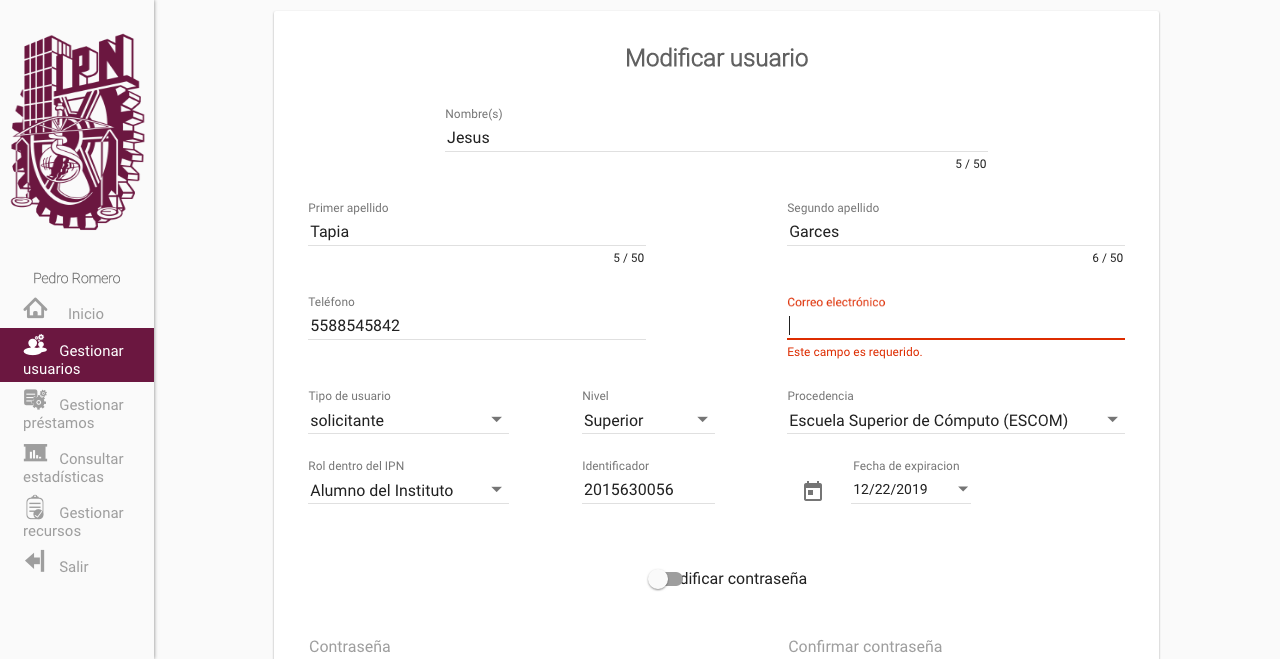
\includegraphics[scale=0.3]{images/Interfaz/MAT-18 Datos incompletos2.png}
	\caption{Datos incompletos}
	\end{figure}
\end{enumerate}

\subsection{Subpaso 2-D: No se pudo recuperar un elemento}
\begin{enumerate}
	\item Seleccione la opción de \textbf{Aceptar} del mensaje
\textbf{MAT-52 Error al cargar la página}.
	\item Ingrese de nuevo desde la interfaz 
\textbf{IUGS-00 Login}.
\end{enumerate}

\subsection{Subpaso 2-E: Error en formato de contraseña}
\begin{enumerate}
	\item Seleccione la opción de \textbf{Aceptar} del mensaje
\textbf{MAT-30 Error en el formato de la contraseña}.
	\item Seleccione otra contraseña con el formato correcto.
	\begin{figure}[hbtp]
	\includegraphics[scale=0.3]{images/Interfaz/MAT-30 Error en el formato de la contraseña.png}
	\caption{Error en el formato de la contraseña}
	\end{figure}
\end{enumerate}

\subsection{Subpaso 2-F: Error en coincidencia de contraseñas}
\begin{enumerate}
	\item Seleccione la opción de \textbf{Aceptar} del mensaje
\textbf{MAT-31 La confirmación de contraseña no coincide}.
	\item Vuelva a escribir la contraseña para que coincida con la previamente elegida.
	\begin{figure}[hbtp]
	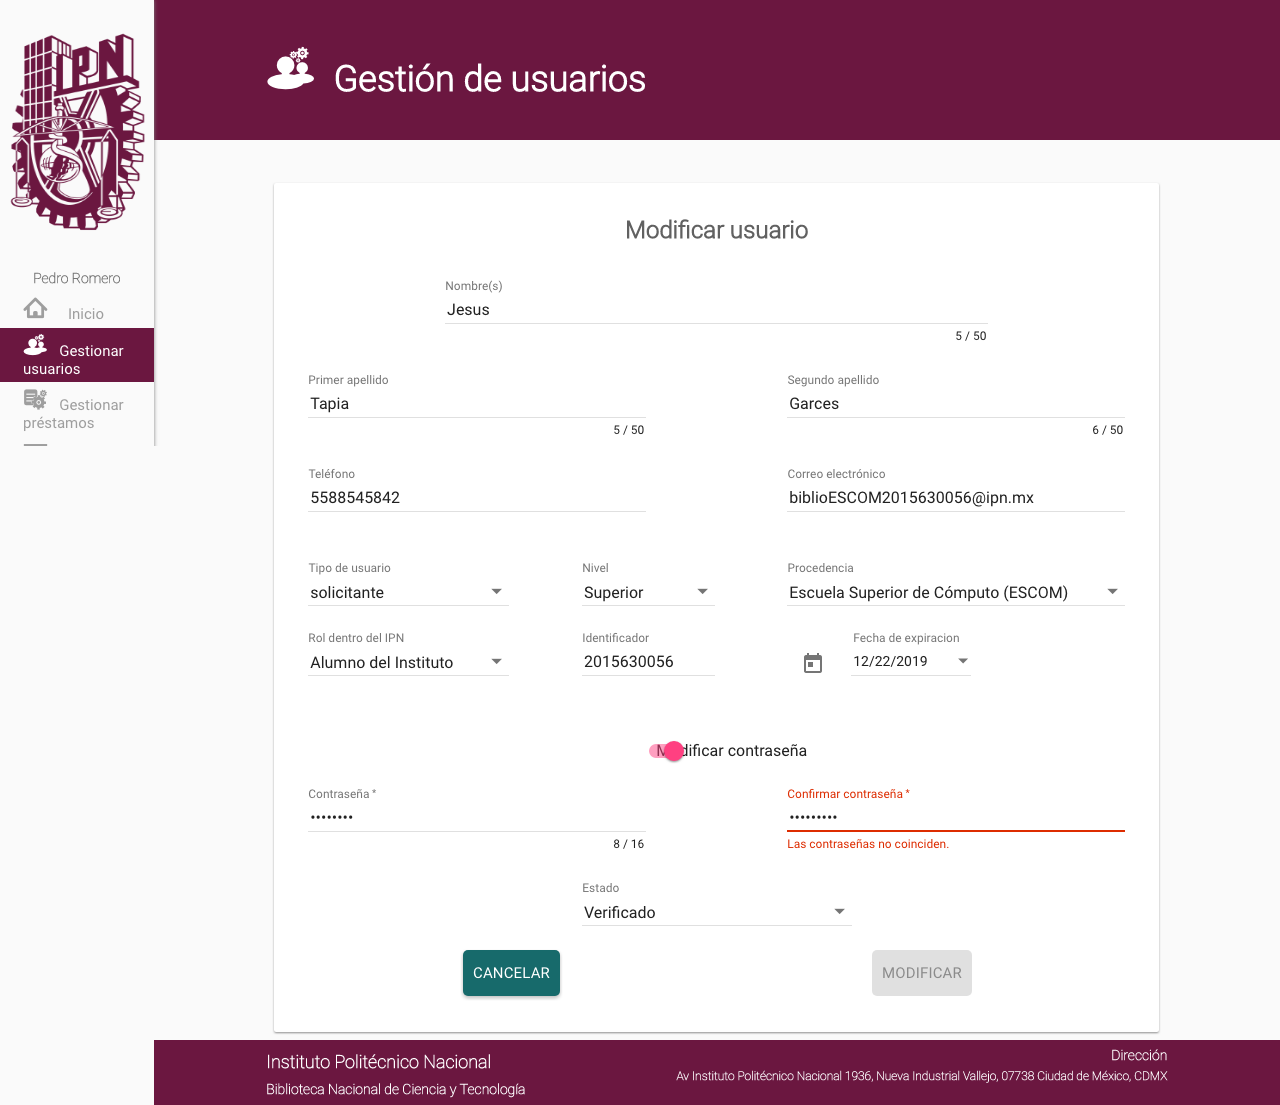
\includegraphics[scale=0.3]{images/Interfaz/MAT-31 La confirmación de contraseña no coincide.png}
	\caption{La confirmación de contraseña no coincide}
	\end{figure}
\end{enumerate}

\subsection{Subpaso 2-G: Error en formato de nombre de usuario}
\begin{enumerate}
	\item Seleccione la opción de \textbf{Aceptar} del mensaje
\textbf{MAT-20 Nombre con formato erróneo}.
	\item Seleccione otro nombre de usuario con el formato correcto.
	\begin{figure}[hbtp]
	\includegraphics[scale=0.3]{images/Interfaz/MAT-20 Nombre con formato erróneo.png}
	\caption{Nombre con formato erróneo}
	\end{figure}
\end{enumerate}

\subsection{Subpaso 2-H: Error en formato de primer apellido}
\begin{enumerate}
	\item Seleccione la opción de \textbf{Aceptar} del mensaje
\textbf{MAT-21 primer apellido con formato erróneo}.
	\item Seleccione otro primer apellido con el formato correcto.
	\begin{figure}[hbtp]
	\includegraphics[scale=0.3]{images/Interfaz/MMAT-21 primer apellido con formato erróneo.png}
	\caption{primer apellido con formato erróneo}
	\end{figure}
\end{enumerate}

\subsection{Subpaso 2-I: Error en formato de segundo apellido}
\begin{enumerate}
	\item Seleccione la opción de \textbf{Aceptar} del mensaje
\textbf{MAT-22 segundo apellido con formato erróneo}.
	\item Seleccione otro segundo apellido con el formato correcto.
	\begin{figure}[hbtp]
	\includegraphics[scale=0.3]{images/Interfaz/MAT-22 segundo apellido con formato erróneo.png}
	\caption{segundo apellido con formato erróneo}
	\end{figure}
\end{enumerate}

\subsection{Subpaso 2-J: Error en formato de teléfono}
\begin{enumerate}
	\item Seleccione la opción de \textbf{Aceptar} del mensaje
\textbf{MAT-23 Teléfono del usuario incorrecto}.
	\item Seleccione otro teléfono con el formato correcto.
	\begin{figure}[hbtp]
	\includegraphics[scale=0.3]{images/Interfaz/MAT-23 Teléfono del usuario incorrecto.png}
	\caption{Teléfono del usuario incorrecto}
	\end{figure}
\end{enumerate}

\subsection{Subpaso 2-K: Error en formato de correo electrónico}
\begin{enumerate}
	\item Seleccione la opción de \textbf{Aceptar} del mensaje
\textbf{MAT-24 Formato de correo electrónico del usuario inválido}.
	\item Seleccione otro correo electrónico con el formato correcto.
	\begin{figure}[hbtp]
	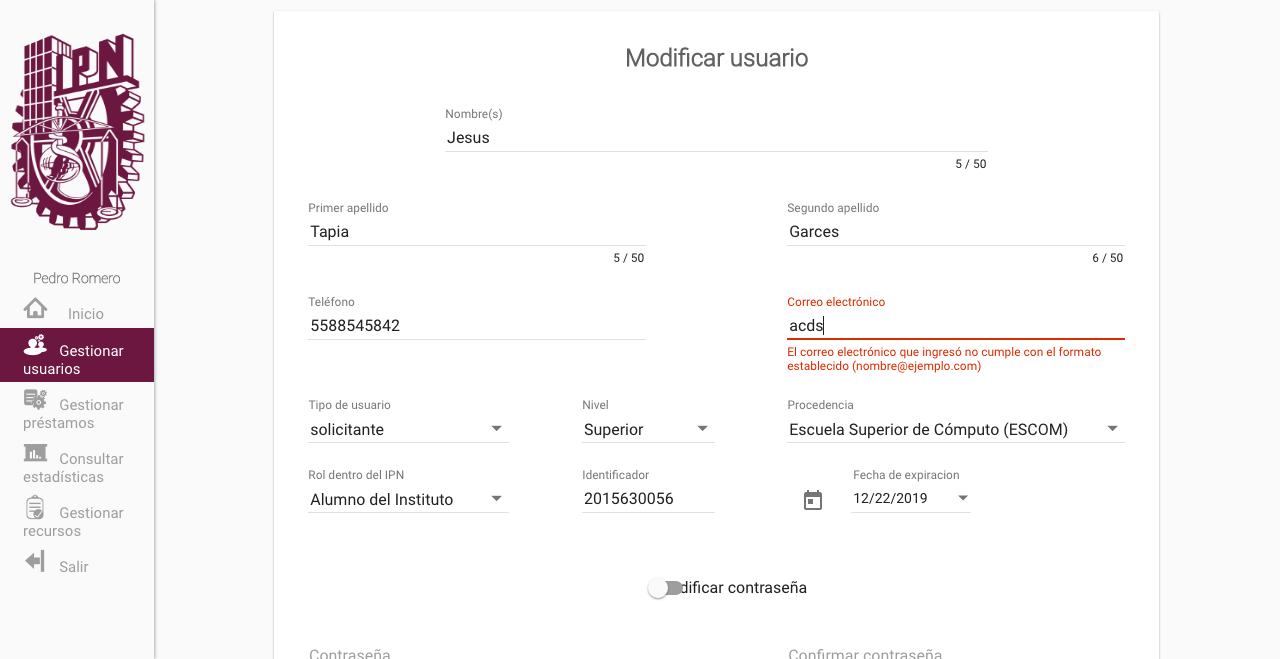
\includegraphics[scale=0.3]{images/Interfaz/MAT-24 Formato de correo electrónico del usuario inválido.png}
	\caption{Formato de correo electrónico del usuario inválido}
	\end{figure}
\end{enumerate}

\subsection{Subpaso 2-L: Usuario ya registrado}
\begin{enumerate}
	\item Seleccione la opción de \textbf{Aceptar} del mensaje
\textbf{MAT-17 Usuario ya registrado}.
	\item Seleccione otro identificador de usuario que no esté registrado.
\end{enumerate}

\subsection{Subpaso 2-M: Fecha de expiración errónea}
\begin{enumerate}
	\item Seleccione la opción de \textbf{Aceptar} del mensaje
\textbf{MAT-47 Fecha de expiración no válida}.
	\item Seleccione otra fecha de expiración posterior al día en curso.
	\begin{figure}[hbtp]
	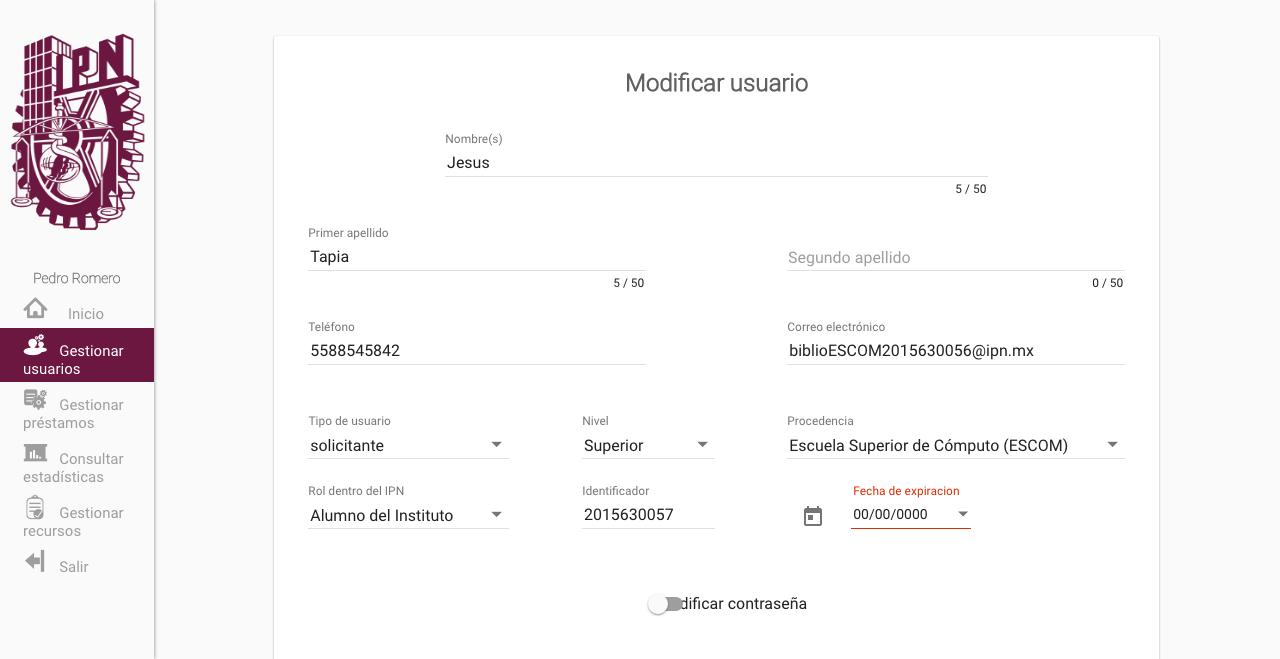
\includegraphics[scale=0.3]{images/Interfaz/MAT-47 Fecha de expiración no válida.png}
	\caption{Fecha de expiración no válida}
	\end{figure}
\end{enumerate}

\subsection{Subpaso 2-N: Modificar usuario de tipo solicitante}
\begin{enumerate}
	\item Ingrese la nueva fecha de vigencia del usuario como comunidad politécnica.
\item Siga completando los campos necesarios.
\end{enumerate}

\subsection{Subpaso 2-O: Usuario con dos apellidos}
\begin{enumerate}
	\item Ingrese el segundo apellido.
\item Siga completando los campos necesarios.
\end{enumerate}

\subsection{Subpaso 2-P: Identificador de usuario incorrecto}
\begin{enumerate}
	\item \item Seleccione la opción de \textbf{Aceptar} del mensaje
\textbf{MAT-50 Identificador inválido}.
	\item Ingrese un identificador válido y continúe completando los campos necesarios.
	\begin{figure}[hbtp]
	\includegraphics[scale=0.3]{images/Interfaz/MAT-50 Identificador inválido2.png}
	\caption{Identificador inválido}
	\end{figure}
\end{enumerate}
